%externalize tikz
\usetikzlibrary{external}
\tikzexternalize[prefix=licht/tikz/, figure name=plot]

%used for drawing n(r)-Area
\definecolor{lGray}{gray}{0.8}
\definecolor{llGray}{gray}{0.9}
\usepgfplotslibrary{fillbetween}

\tikzset{
  ring shading/.code args={from #1 at #2 to #3 at #4}{
    \def\colin{#1}
    \def\radin{#2}
    \def\colout{#3}
    \def\radout{#4}
    \pgfmathsetmacro{\proportion}{\radin/\radout}
    \pgfmathsetmacro{\outer}{.8818cm}
    \pgfmathsetmacro{\inner}{.8818cm*\proportion}
    \pgfmathsetmacro{\innerlow}{\inner-0.01pt}
    \pgfdeclareradialshading{ring}{\pgfpoint{0cm}{0cm}}%
    {
      color(0pt)=(white);
      color(\innerlow)=(white);
      color(\inner)=(#1);
      color(\outer)=(#3)
    }
    \pgfkeysalso{/tikz/shading=ring}
  },
}

%\usepackage{subcaption}
%\usepackage{subfigure}
    
\chapter{Lichtbrechung in der Atmosph"are\label{chapter:thema}}
\lhead{Lichtbrechung in der Atmosph"are}
\begin{refsection}
\chapterauthor{Simon Schaefer und Tibor Schneider}

\printbibliography[heading=subbibliography]
\end{refsection}

%polar plot
\usepgfplotslibrary{polar}

\section{Einleitung}
Der Blick an den Nachthimmel fasziniert uns Menschen schon seit Jahrtausenden. "Ahnlich der Frage "uber das Leben nach dem Tod wurden damit ganze Religionen und Kulturen begr"undet beziehungsweise zugrunde gerichtet. 
"Uber die Jahrhunderte wuchs die Einsicht, wenn auch nicht stetig und leider auch nicht strikt monoton, dass eine genauere Vermessung des Nachthimmels, die Astrometrie, wenigstens physikalische Grundlagen zur Diskussion betragen kann. 
W"ahrend Galileo Galilei noch mit blossem Auge und einem besseren Flaschenboden den Nachhimmel beobachtete (TODO: QUELLE), nutzte T. Brahe bereits ein XXX Teleskop (TODO: QUELLE). 
Beide beobachteten die Bewegungen der Planeten unseres Sonnensystems und nahmen die Positionen entfernterer Sterne, Galaxien und anderen Objekten als sogenannte Fixsterne als konstant an. 
W"ahrend die Nasa und andere noch daran t"ufteln einen Menschen auf unseren n"achsten Nachbarplaneten zu bugsieren, sind unsere Blicke und v.a. unsere Neugier bereits Milliarden von Lichtjahren "uber unser Sonnensystem hinaus ins Weltall gerichtet. 
Die ehemaligen Fixsterne sind zu dynamischen Konstallationen erstaunlicher Ph"anomene geworden.
Neue Technologien der Sensorik erz"ahlen uns von der materiellen Zusammensetzung leuchtender Gaswolken. 
Gewaltige Pulsare werden zu Meilensteinen intergalaktischen Kartographie. 
Die Bewegung und die unfassbaren Distanzen ganzer Galaxien von unserem Heimatplaneten geben uns sogar die M"oglichkeit in der Zeit zur"uck zu blicken.
Die Gr"osse unseres Universums  erlaubt es sogar Annahmen "uber das Schicksal unseres eigenen Sonnensystems zu treffen, indem wir andere Systeme beobachten. 
Die extremen Distanzen zwischen uns und den beobachteten Objekten fordern eine hohe Pr"azision bei der Konstruktion der verwendeten Messinstrumente sowie ein tiefes Verst"andnis aller mo"glichen Effekte, die unseren Blick in die Tiefe des Weltalls beeinflussen. 
Angefangen bei simplen Regenwolken, "uber die Lichtverschmutzung unserer Zivilisation, zu optischen Effekten der Lichtbrechung in der Atmosph"are durch die Temperatur und Zusammensamensetzung, ja sogar Bewegung der Lufschichten bis hin zu relativistischen Effekten (TODO: QUELLE), die einen Lichtstrahl aus weiter Ferne so manipulieren k"onnen, dass uns dessen Ursprung an ganz anderem Ort erscheint, als er tats"achlich ist. 
Schon in der Primarschule lehr der Strahlensatz, dass schon kleine Messfehler bei der Auswertung eines Bildes hier auf der Erde, hochgerechnet auf die Weiten des Universums extreme Dimensionen annehmen. (TODO: HISTORISCHES BEISPIEL). 
In diesem Artikel m"ochten wir nun basierend auf Jean Kovalevsky und P. Kenneth Seidelmanns 6. Kapitel in Grundlagen der Astrometrie \cite{licht:astrometry} die scheinbare Verschiebung beobachteter Objekte und deren mathematischen Korrektur beschreiben. 

\section{Planares Modell} 
\begin{figure}
\centering
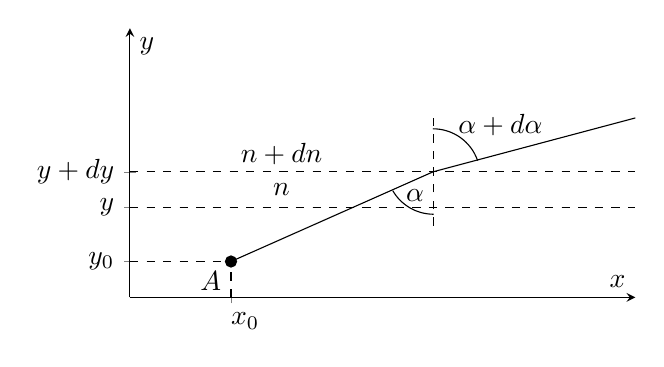
\begin{tikzpicture}
  \begin{axis}[xlabel=$x$, ylabel = $y$, axis lines=middle, height=5cm, width = 8cm,
  ymin=0, ymax=1.5, xmin=0, xmax=1, yticklabels={$y_0$, $y$, $y + dy$}, ytick =
  {0.2,0.5,0.7}, xtick={0.2}, xticklabel={\rlap{$x_0$}}]
    \draw[dashed] (axis cs:0,0.5) -- (axis cs:1,0.5);
    \draw[dashed] (axis cs:0,0.7) -- (axis cs:1,0.7);
    \draw[dashed] (axis cs:0,0.5) -- (axis cs:1,0.5);
    \draw[dashed] (axis cs:0.2,0) -- (axis cs:0.2,0.2);
    \draw[dashed] (axis cs:0,0.2) -- (axis cs:0.2,0.2);
    \filldraw (axis cs:0.2,0.2) circle (2pt) node[anchor=north east] {$A$};
    \draw (axis cs:0.2,0.2) -- (axis cs:0.6,0.7);
    \draw (axis cs:0.6,0.7) -- (axis cs:1,1);
    \draw (axis cs:0.52, 0.595) arc (210:270:0.6cm) node[anchor=north east, yshift =
    +0.44cm] {$\alpha$};
    \draw (axis cs:0.688,0.762) arc (19:90:0.6cm) node[anchor=west, yshift=+0.05cm,
    xshift=+0.2cm] {$\alpha + d\alpha$};  
    \draw[dashed](axis cs:0.6,0.4) -- (axis cs:0.6,1);
    \draw (axis cs:0.3, 0.6) node {$n$};
    \draw (axis cs:0.3, 0.8) node {$n + dn$};
  \end{axis}
\end{tikzpicture}
\caption{Skizze des planaren Modells}
\label{fig:13_1}
\end{figure}


F"ur die Herleitung des Weges, welcher der Lichtstrahl zurücklegt, gehen wir von Snell's Law aus: $n_1 \sin \alpha_1 = n_2 \sin \alpha_2$.
Mit der in der Grafik verwendeten Notation:

\begin{equation} \label{eq:13_1}
  n \cdot \sin(\alpha) = n_0 \cdot \sin(\alpha_0) = \varepsilon
\end{equation}

Aus der Geometrie in der Abbildung \ref{fig:13_1} ist ersichtlich:
$$\frac{\cos \alpha}{\sin \alpha} = \frac{dy}{dx} = y'(x)$$
$$\Rightarrow y'(x)^2 = \frac{1 - \sin^2 \alpha}{\sin^2 \alpha} = \frac{1}{\sin^2 \alpha} - 1$$

Nun k"onnen wir das nach $sin^2(\alpha)$ aufl"osen, indem wir durch $y'(x)^2$ teilen. 
Da dies möglicherweise gleich Null sein kann, muss dieser Fall separat behandelt werden (siehe Kapitel \ref{ch:spezialfall}). 
Von nun an gilt die Bedingung: $y'(x) \neq 0$.

\begin{equation} \label{eq:13_2}
\sin^2 (\alpha) = \frac{1}{y'(x)^2 + 1}
\end{equation}

Nun quadrieren wir die Gleichung \ref{eq:13_1}, setzen \ref{eq:13_2} ein und l"osen nach $y'(x)$ auf:

$$n^2 \cdot \frac{1}{y'(x)^2 + 1} = \varepsilon^2 = (n_0 \cdot \sin \alpha_0)^2$$

Nun k"onnte man diese Differentialgleichung erster Ordnung nummerisch lösen. 
Das Problem jedoch ist, dass die Anfangssteigung $y'(0)$ in der Gleichung in Form von $\alpha_0 = \arctan (y'(0))$ vorliegt. Das die Differentialgleichung in der ersten Ordnung vorliegt, k"onnen wir sie nach $x$ ableiten, und erhalten somit:

$$\frac{d}{dx} \left( \frac{n^2}{y'^2 + 1} \right) = \frac{2n}{y'^4 + 2y'^2 + 1} \cdot \left( n'(y'^2 + 1) - n y' y'' \right) = 0$$

Da $n(y(x))$ abh"angt, wird in diesen Formeln die Notation $n'_r = \frac{dn}{dr}$ verwendet.
Nun ist $\alpha_0$ nicht mehr vorhanden und die jetzt vorliegende Gleichung hat Ordnung 2. 
Der Anfangswinkel ist nun teil der Anfangsbedingung. 
Da der ganze Term gleich 0 ist, muss der Ausdruck in den Klammern gleich 0 sein:

$$n' y'^2 + n' - n y' y'' = 0$$
$$y''(x) = \frac{n'_r (y(x))}{n(y(x))} \cdot \left( y'(x) + \frac{1}{y'(x)} \right)$$

Aufgrund der Kettenregel $\frac{dn}{dx} = \frac{dn}{dy} \cdot \frac{dy}{dx}$ kann man die Differentialgleichung weiter vereinfachen. 

\begin{equation} \label{eq:planar_DGL}
y''(x) = \frac{\frac{dn}{dy}}{n(y)} \cdot \left( y'(x)^2 + 1\right) = \frac{n'_y}{n}
\end{equation}

\subsection{Vergleichsgr"osse $\Delta \alpha$}
Um die Resultate vergleichen zu k"onnen, brauchen wir ein Mass f"ur die Brechung. 
Wir definieren $\Delta \alpha$ als die Änderung des Winkels der Funktion am Anfang und dort, wo sie nicht mehr weiter gebrochen wird (siehe Abbildung \ref{fig:skizze_mass}). Diese Gr"osse wird sowie im Planaren, als auch im Sph"arischen Modell verwendet. 

\begin{figure}
  \centering
  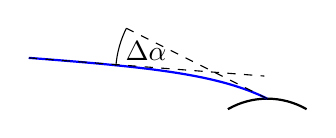
\begin{tikzpicture}
    \draw [thick] (60:1) arc (60:120:1);
    \draw [blue, thick] plot [smooth] coordinates {(0.00000,1.00000)(-0.02913,1.01430)(-0.05912,1.02850)(-0.09001,1.04260)(-0.12186,1.05660)(-0.15622,1.07112)(-0.19174,1.08553)(-0.22848,1.09983)(-0.26652,1.11403)(-0.30594,1.12812)(-0.34683,1.14210)(-0.38928,1.15598)(-0.43341,1.16975)(-0.47931,1.18342)(-0.52714,1.19699)(-0.57702,1.21047)(-0.62912,1.22384)(-0.68363,1.23713)(-0.74072,1.25033)(-0.80064,1.26345)(-0.86364,1.27649)(-0.93000,1.28947)(-1.00004,1.30239)(-1.07415,1.31527)(-1.15276,1.32813)(-1.23636,1.34098)(-1.32554,1.35386)(-1.42096,1.36679)(-1.52345,1.37982)(-1.63395,1.39301)(-1.75359,1.40640)(-1.88375,1.42009)(-2.02615,1.43419)(-2.18287,1.44884)(-2.35647,1.46418)(-2.55025,1.48045)(-2.76851,1.49798)(-3.02833,1.51805)};
    \draw [dashed] (0,1) -- ++(153.43:2);
    \draw [dashed] (-3.02833,1.51805) -- ++(-4.417:3);
    \draw (133.356:2.6056) arc (153.43:175.583:1.3) node [above right, yshift=-0.5mm] {$\Delta \alpha$}; 
  \end{tikzpicture}
  \caption{Skizze des Mass der Kr"ummung $\Delta \alpha$. \label{fig:skizze_mass}}
\end{figure}


\subsection{Verifikation}
Um zu "uberpr"ufen, ob unser Modell plausibel ist, setzen wir verschiedene Funktionen f"ur $n(y)$ ein. 
Wenn die Brechzahl konstant ist (das Heisst $\frac{dn}{dy} = 0$), dann sollte der Lichtstrahl nicht mehr gebrochen werden und auf einer Geraden weiterfahren. 
Wenn man nun $n'(y)=0$ in die Gleichung \ref{eq:planar_DGL} einsetzt, erhält man: 

$$y''(x) = 0$$

Auch aus unserer Gleichung ist also erkennbar, dass sich der Lichtstrahl bei konstantem $n$ nicht bricht.

Nun brauchen wir eine Funktion der Brechzahl in Abh"angigkeit der H"ohe. 
Der Brechungsindex der Luft h"angt (teilweise) vom Druck ab. 
Der H"ohendruck von Gasen nimmt nach der barometrischen H"ohenformel (TODO:QUELLE) mit der H"ohe exponentiell ab.

Ausserdem ist die Brechzahl immer $n \geq 1$, wobei im Vakuum $n=1$ gilt. 
Mit diesen Informaitonen stellen wir die Brechzahl folgendermassen dar:

$$n(y) = 1 + \mu e^{- \sigma y}, \qquad \frac{dn}{dy} = -\sigma \mu \cdot e^{-\sigma y}$$

Nun setzen wir dies in die Differentialgleichung ein, und erhalten:

\begin{equation} \label{eq:planar_DGL_n}
y''(x) = \frac{-\sigma}{\frac{1}{\mu e^{-\sigma y}} + 1} \cdot \left( y'(x)^2 + 1 \right)
\end{equation}

Der Lichtstrahl sollte sich immer in richtung des gr"osseren $n$ kr"ummen. 
Bei unserer Funktion bedeutet dies, er kr"ummt sich nach unten. 
Um dies besser darzustellen, wird die Brechzahl in den Grafiken Grau eingezeichnet.
Diese Differentialgleichung lässt sich nummerisch l"osen (siehe Abbildung \ref{fig:planares_modell1}).
Wie zu erwarten war, kr"ummen sich die Lichtstrahlen nach unten.
Je H"oher der Strahl ist, desto schw"acher kr"ummt er sich. 

\begin{figure}
  \centering
  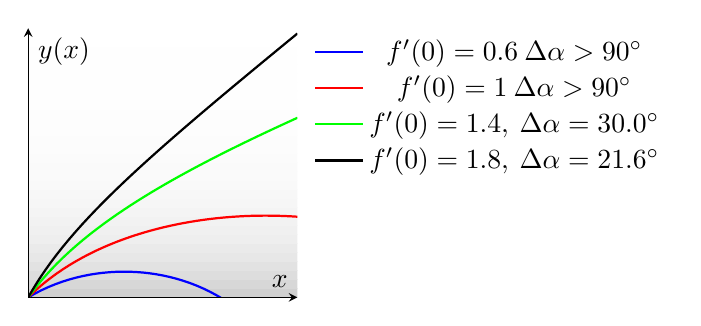
\begin{tikzpicture}
    \begin{axis}[xlabel=$x$, ylabel=$y(x)$, axis lines=middle, height=5cm, width=5cm, ticks
    = none, legend pos = outer north east, legend style={draw=none}, ymin = 0, ymax = 10,
    xmin = 0, xmax = 10, colormap={traditionalpm3d}{color=(white) color=(lGray)}, %colorbar,
    view={0}{90}] 

    \addplot3[surf, domain=-10:10, y domain=0:20 , shader=flat, samples=61, forget plot] {1 + 1 * exp(-y/2)};  
    %\addlegendentry{$n(y)$}
  
    \addplot [mark = none, thick, draw=blue] coordinates{
        (0.00000,0.00000)(0.00008,0.00005)(0.00017,0.00010)(0.00025,0.00015)
        (0.00033,0.00020)(0.00075,0.00045)(0.00117,0.00070)(0.00159,0.00095)
        (0.00201,0.00121)(0.00410,0.00246)(0.00620,0.00371)(0.00829,0.00496)
        (0.01038,0.00622)(0.02085,0.01245)(0.03131,0.01866)(0.04178,0.02485)
        (0.05225,0.03100)(0.10458,0.06137)(0.15691,0.09107)(0.20924,0.12012)
        (0.26157,0.14852)(0.51157,0.27569)(0.76157,0.38962)(1.01157,0.49129)
        (1.26157,0.58151)(1.51157,0.66092)(1.76157,0.73009)(2.01157,0.78945)
        (2.26157,0.83938)(2.51157,0.88018)(2.76157,0.91208)(3.01157,0.93526)
        (3.26157,0.94986)(3.51157,0.95594)(3.76157,0.95354)(4.01157,0.94265)
        (4.26157,0.92322)(4.51157,0.89512)(4.76157,0.85822)(5.01157,0.81229)
        (5.26157,0.75706)(5.51157,0.69221)(5.76157,0.61731)(6.01157,0.53186)
        (6.26157,0.43525)(6.51157,0.32674)(6.76157,0.20546)(7.01157,0.07031)
        (7.26157,-0.08007)(7.51157,-0.24736)(7.76157,-0.43357)(8.01157,-0.64143)
        (8.26157,-0.87451)(8.51157,-1.13773)(8.76157,-1.43704)(9.01157,-1.78220)
        (9.26157,-2.18838)(9.40485,-2.45726)(9.54812,-2.76003)(9.69140,-3.10717)
        (9.83468,-3.51505)(9.87601,-3.64716)(9.91734,-3.78722)(9.95867,-3.93632)
        (10.00000,-4.09576)};
    \addlegendentry{$f'(0) = 0.6 \: \Delta \alpha > 90^\circ$}
    
    \addplot [mark = none, thick, draw=red] coordinates{
        (0.00000,0.00000)(0.00005,0.00005)(0.00010,0.00010)(0.00015,0.00015)
        (0.00020,0.00020)(0.00045,0.00045)(0.00070,0.00070)(0.00095,0.00095)
        (0.00121,0.00121)(0.00246,0.00246)(0.00372,0.00372)(0.00497,0.00497)
        (0.00623,0.00622)(0.01251,0.01248)(0.01879,0.01872)(0.02507,0.02495)
        (0.03135,0.03117)(0.06275,0.06202)(0.09415,0.09252)(0.12554,0.12267)
        (0.15694,0.15248)(0.31394,0.29668)(0.47093,0.43331)(0.62792,0.56302)
        (0.78491,0.68641)(1.03491,0.87100)(1.28491,1.04240)(1.53491,1.20197)
        (1.78491,1.35087)(2.03491,1.49003)(2.28491,1.62024)(2.53491,1.74218)
        (2.78491,1.85645)(3.03491,1.96356)(3.28491,2.06393)(3.53491,2.15797)
        (3.78491,2.24601)(4.03491,2.32835)(4.28491,2.40526)(4.53491,2.47697)
        (4.78491,2.54370)(5.03491,2.60563)(5.28491,2.66293)(5.53491,2.71574)
        (5.78491,2.76420)(6.03491,2.80844)(6.28491,2.84854)(6.53491,2.88461)
        (6.78491,2.91672)(7.03491,2.94495)(7.28491,2.96936)(7.53491,2.98999)
        (7.78491,3.00690)(8.03491,3.02011)(8.28491,3.02966)(8.53491,3.03557)
        (8.78491,3.03784)(9.03491,3.03648)(9.28491,3.03149)(9.53491,3.02286)
        (9.78491,3.01056)(9.83869,3.00744)(9.89246,3.00414)(9.94623,3.00068)
        (10.00000,2.99704)};
    \addlegendentry{$f'(0) = 1 \: \Delta \alpha > 90^\circ$}
    
    \addplot [mark = none, thick, draw=green] coordinates{
       (0.00000,0.00000)(0.00004,0.00005)(0.00007,0.00010)(0.00011,0.00015)
       (0.00014,0.00020)(0.00032,0.00045)(0.00050,0.00070)(0.00068,0.00095)
       (0.00086,0.00121)(0.00176,0.00246)(0.00266,0.00372)(0.00355,0.00497)
       (0.00445,0.00622)(0.00894,0.01249)(0.01342,0.01874)(0.01791,0.02498)
       (0.02239,0.03121)(0.04482,0.06220)(0.06725,0.09292)(0.08967,0.12337)
       (0.11210,0.15358)(0.22424,0.30091)(0.33638,0.44255)(0.44852,0.57900)
       (0.56065,0.71072)(0.81065,0.98925)(1.06065,1.24961)(1.31065,1.49459)
       (1.56065,1.72638)(1.81065,1.94668)(2.06065,2.15691)(2.31065,2.35825)
       (2.56065,2.55168)(2.81065,2.73803)(3.06065,2.91802)(3.31065,3.09225)
       (3.56065,3.26128)(3.81065,3.42555)(4.06065,3.58549)(4.31065,3.74145)
       (4.56065,3.89376)(4.81065,4.04271)(5.06065,4.18856)(5.31065,4.33154)
       (5.56065,4.47186)(5.81065,4.60971)(6.06065,4.74527)(6.31065,4.87869)
       (6.56065,5.01012)(6.81065,5.13969)(7.06065,5.26753)(7.31065,5.39374)
       (7.56065,5.51843)(7.81065,5.64170)(8.06065,5.76362)(8.31065,5.88429)
       (8.56065,6.00378)(8.81065,6.12216)(9.06065,6.23950)(9.31065,6.35585)
       (9.56065,6.47128)(9.67049,6.52171)(9.78033,6.57198)(9.89016,6.62209)
       (10.00000,6.67204) };
    \addlegendentry{$f'(0) = 1.4, \: \Delta \alpha = 30.0^\circ$}
    
    \addplot [mark = none, thick, draw=black] coordinates{
       (0.00000,0.00000)(0.00003,0.00005)(0.00006,0.00010)(0.00008,0.00015)
       (0.00011,0.00020)(0.00025,0.00045)(0.00039,0.00070)(0.00053,0.00095)
       (0.00067,0.00121)(0.00137,0.00246)(0.00207,0.00372)(0.00276,0.00497)
       (0.00346,0.00622)(0.00695,0.01249)(0.01044,0.01875)(0.01393,0.02499)
       (0.01742,0.03123)(0.03486,0.06227)(0.05230,0.09308)(0.06975,0.12366)
       (0.08719,0.15403)(0.17441,0.30265)(0.26163,0.44635)(0.34885,0.58556)
       (0.43606,0.72069)(0.64497,1.02972)(0.85387,1.32103)(1.06278,1.59761)
       (1.27168,1.86179)(1.52168,2.16416)(1.77168,2.45381)(2.02168,2.73271)
       (2.27168,3.00247)(2.52168,3.26436)(2.77168,3.51946)(3.02168,3.76864)
       (3.27168,4.01267)(3.52168,4.25218)(3.77168,4.48771)(4.02168,4.71973)
       (4.27168,4.94865)(4.52168,5.17481)(4.77168,5.39853)(5.02168,5.62008)
       (5.27168,5.83969)(5.52168,6.05756)(5.77168,6.27389)(6.02168,6.48883)
       (6.27168,6.70254)(6.52168,6.91513)(6.77168,7.12672)(7.02168,7.33741)
       (7.27168,7.54730)(7.52168,7.75647)(7.77168,7.96499)(8.02168,8.17292)
       (8.27168,8.38032)(8.52168,8.58724)(8.77168,8.79374)(9.02168,8.99986)
       (9.27168,9.20562)(9.45376,9.35529)(9.63584,9.50480)(9.81792,9.65416)
       (10.00000,9.80340) };
    \addlegendentry{$f'(0) = 1.8, \: \Delta \alpha = 21.6^\circ$}
    
  
    \end{axis}
  \end{tikzpicture}
  \caption{Nummerische L"osung der Differentialgleichung (\ref{eq:planar_DGL_n}). \label{fig:planares_modell1}}

\end{figure}

TODO: M"oglicherweise weitere Brechzahlen "uberpr"ufen

\subsection{Spezialfall: $y'(x) = 0$} \label{ch:spezialfall}

In diesem Modell ist die Brechzahl $n$ nur von $y$ abhängig. 
Falls die Funktion nun die Steigung $f'(x) = 0$ hat, dann "andert sich die Brechzahl in Richtung des Lichtstrahls nicht mehr.
Dies w"urde bedeuten, dass sich der Lichtstrahl nicht weiter kr"ummt. 

In der Realit"at gibt es in der Luft immer relativ starke Unregelm"assigkeiten. 
Betrachten wir das Beispiel der Abbildung \ref{fig:planares_modell1}. 
Falls der Lichtstrahl waagerecht ist, kann er aufgrund der Unregelm"assigkeiten entweder nach oben oder unten gebrochen werden. 
Wenn er nach oben gebrochen wird, so kr"ummt er sich sofort wieder nach unten.
Und wenn er sich nach unten bricht, dann kr"ummt er sich weiter nach unten.  
Der Fall $y'(x) = 0$ ist also in diesem Modell kein station"arer Punkt. 
In der Realit"at ist dieser Spezialfall also nicht problematisch. 

In unserem Modell jedoch wird bei der Herleitung durch $y'(x)$ geteilt.
Die Gleichung \ref{eq:planar_DGL} gilt also nicht f"ur diesen Spezialfall. 
Duch den Quantisierungsfehler beim nummerischen L"osen wird jedoch dieser Spezialfall nie erreicht, und wir m"ussen ihn in der Simulation nicht ber"ucksichtigen.
Wie in der Abbildung \ref{fig:planares_modell1} an der blauen Kurve mit $f'(0) = 0.6$ zu erkennen ist, kr"ummt sich der Lichtstrahl weiter.


\section{Sph"arisches Modell}

Wir beginnen erneut mit Snell's Gleichung, welche wir auf unser Sph"arischen Modells (Abbildung \ref{fig:sphere_skizze}) angepasst wurde: 

$$n \cdot \sin \beta = (n + dn) \cdot \sin(\alpha + d\alpha)$$

Im Dreieck $OMN$ l"asst sich mit dem Sinussatz folgende Beziehung herleiten:

$$r \sin\alpha = (r + dr) \cdot \sin\beta$$

Multipliziert man nun die beiden Gleichungen, erh"alt man:

\begin{equation} \label{eq:sphere_base}
n r \sin \alpha = (n + dn)(r + dr) \sin (\alpha + d\alpha) = n_0 r_0 \sin \alpha_0
\end{equation}

Somit sind nicht mehr zwei verschiedene Winkel in der Formel vorhanden.

Wie beim Planaren Modell ist dieses Produkt konstant. 
Wir suchen eine Funktion $r(\varphi))$, welche den Weg eines Lichtstrahls beschreibt, der am Punkt $A$ mit Anfangswinkel $\alpha_0$ startet (oder dort dendet). 

Aus dem Dreieck $MNP$ kann folgende Beziehung hergeleitet werden:

$$\tan \alpha =  \frac{\overline{NP}}{\overline{MP}} = \frac{r \cdot d\varphi}{dr} = \frac{r}{\frac{dr}{d\varphi}} = \frac{r}{r'}$$

Wir quadrieren die diese Gleichung und l"osen nach $\sin^2(\beta)$ auf:

$$\tan^2 \alpha = \frac{\sin^2\alpha}{\cos^2\alpha} = \frac{\sin^2\alpha}{1-\sin^2\alpha} = \frac{1}{\frac{1}{\sin^2\alpha}-1} \left( \frac{r(\varphi)}{r'(\varphi)} \right)^2$$

\begin{equation} \label{eq:sphere_sine}
\Rightarrow \sin^2\alpha = \frac{1}{\left( \frac{r'(\varphi)}{r(\varphi)} \right)^2 +1}
\end{equation}

\begin{figure} 
\centering
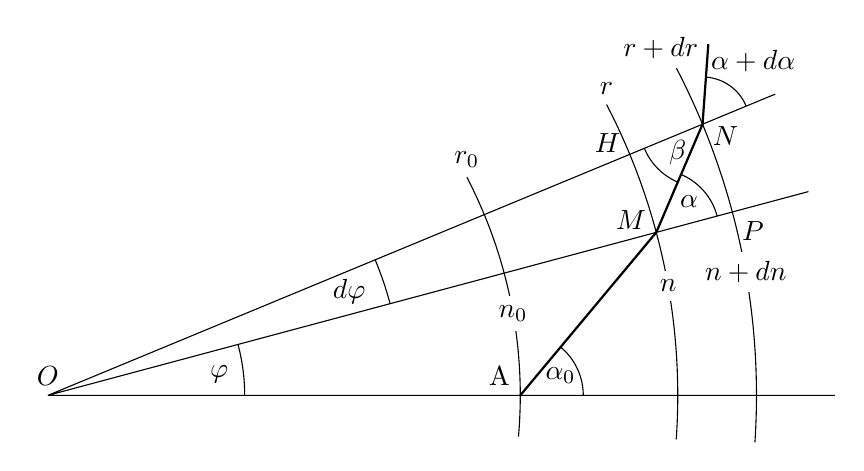
\begin{tikzpicture}
  %radial lines
  \draw (0,0) node[above]{$O$} 
        -- ++(0:10cm)
        (0,0) -- ++(15:10cm)
        (0,0) -- ++(22.5:10cm);
  %Radius r0, r, r + dr      
  \draw ([shift=(-5:6cm)]0,0) arc (-5:27.5:6cm) node [above] {$r_0$}
        ([shift=(-4:8cm)]0,0) arc (-4:27.5:8cm) node [above] {$r$}
        ([shift=(-3.8:9cm)]0,0) arc (-3.8:27.5:9cm) node [above, xshift=-0.2cm] {$r +
        dr$};
  %path of the light
  \draw [thick] (0:6cm) node [above left]{A}
        -- (15:8cm) node [above left, yshift=-0.1cm] {$M$}
        -- (22.5:9cm) node [below right, yshift=0.1cm]{$N$}
        -- (28:9.5cm);
  \draw (22.5:8cm) node [above left, yshift=-0.1cm] {$H$};
  \draw (15:9cm) node[below right] {$P$};
  %angles
  \draw ([shift=(-157.5:0.8cm)]22.5:9cm) arc (-157.5:-113.2:0.8cm) node [above,
          yshift=0.1cm]{$\beta$}
        ([shift=(15:0.8cm)]15:8cm) arc (15:66.8:0.8cm) node [below,
          yshift = -0.15cm, xshift=0.1cm]{$\alpha$}
        ([shift=(22.5:0.6cm)]22.5:9cm) arc (22.5:85.9:0.6cm) node
          [xshift=0.6cm, yshift=0.2cm]{$\alpha+d\alpha$}
        ([shift=(0:0.8cm)]0:6cm) arc (0:50.2:0.8cm) node [below,
          yshift=-0.14cm]{$\alpha_0$}
        ([shift=(0:2.5cm)]0,0) arc (0:15:2.5cm) node [below left,
          yshift=-0.15cm]{$\varphi$}
        ([shift=(15:4.5cm)]0,0) arc (15:22.5:4.5cm) node [below left,
          yshift=-0.12cm]{$d\varphi$};
  %refraction rates
  \draw (10:6cm) node[fill=white] {$n_0$}
        (10:8cm) node[fill=white] {$n$}
        (10:9cm) node[fill=white] {$n + dn$};
        
\end{tikzpicture}
\caption{Skizze des Sph"arischen Modells. \label{fig:sphere_skizze}}
\end{figure}

W"ahrend diesen Umformungen wurde durch $r'(\varphi)$ geteilt. 
In den folgenden Gleichungen sei Vorausgesetzt, dass $r'(\varphi) \neq 0$. 
Wie bereits zuvor in Kapitel \ref{ch:spezialfall} beschrieben muss dieser nicht separat behandelt werden.
Nun quadrieren wir die Gleichung \ref{eq:sphere_base} und setzen die Gleichung \ref{eq:sphere_sine} ein:

$$\frac{(n \cdot r(\varphi))^2}{\left( \frac{r'(\varphi)}{r(\varphi)} \right)^2 +1} = (r_0 n_0 \sin \alpha_0)^2$$

Diese Gleichung ist eine Differentialgleichung erster Ordnung. 
Jedoch ist erneut der Term $sin^2(\alpha_0)$ vorhanden, welcher von $r'(\varphi_0)$ abhängt. 
Damit die DGL auch korrekte Anfangsbedingungen erhält, leiten wir die Gleichung nach $\varphi$ ab und erhalten:

$$\frac{d}{d\varphi}\left(\frac{(n r)^2}{\left(\frac{r'}{r}\right)^2 + 1}\right) =  \frac{2 r^2 n r' n'_r}{\frac{r'^2}{r^2}+1}+\frac{2 r n^2 r'}{\frac{r'^2}{r^2}+1}-\frac{r^2 n^2 \left(\frac{2 r' r''}{r^2}-\frac{2 r'^3}{r^3}\right)}{\left(\frac{r'^2}{r^2}+1\right)^2}$$

$$\frac{2n r' r}{\frac{r'^2}{r^2}+1} \cdot \left( n'_r + n - \frac{n r r'' - n r'^2}{r'^2 + r^2} \right) = 0$$

\begin{equation} \label{eq:sphere_origin}
\Rightarrow n'_r + n - \frac{n r r'' - n r'^2}{r'^2 + r^2} = 0
\end{equation}

$$\Rightarrow n'_r r'^2  + n'_r r^2 + n r'^2 + nr^2 = n r r'' - n r'^2$$

$$\Rightarrow n'_r r'^2 + n'_r r^2 + 2 n r'^2 + n r^2 = n r r''$$

\begin{equation} \label{eq:sphere_allg}
\Rightarrow r'' = \frac{n'_r r'^2 + n'_r r^2 + 2 n r'^2 + n r^2}{n r}
\end{equation}

Anmerkung: Da $n(r(\varphi))$ abh"angig von $r(\varphi)$ ist, wird die Notation: $n'_r = \frac{dn}{dr}$ verwendet.

\subsection{Verifikation}
Wie zuvor beim planaren Modell setzen wir verschiedene Funtionen f"ur $n(r)$ ein, und beurteilen die Resultate. 
Als erstes untersuchen wir die Funktion $n(r) = 1, n'(r) = 0$. 
Bei diesem Beispiel hat das Material "uberall dieselbe Brechzahl.
Die Nummerischen L"osungen sollten alle (bez"uglich den karteischen Koordinaten) linear ansteigen und sich nicht kr"ummen. Die Simulation best"atigt dies (siehe Abbildung \ref{fig:sphaerisches_modell1}).

Nun verwenden wir erneut die exponentielle Approximation der Brechzahl: 

$$n(r) = 1 + \mu \cdot e^{-\sigma (r - r_0)} \qquad n'_r(r) = -\sigma \mu e^{-\sigma (r - r_0)}$$

Nun setzen wir dies in die Differentialgleichung \ref{eq:sphere_allg} ein und berechnen die L"osung nummerisch (Abbildung \ref{fig:sphaerisches_modell2}, \ref{fig:sphaerisches_modell3}). 

\begin{figure}
\centering
\begin{tikzpicture}
  \begin{axis} [
    axis lines=none, 
    width=7cm, 
    axis equal,
    ticks = none, 
    legend pos = outer north east, 
    legend style={draw=none}, 
    ymin = 0,
    ymax = 4,
    xmin = -3, 
    xmax = 3, 
  ]
    %f'(0)=1
    \addplot [mark = none, thick, color=red] coordinates {
      (0.00000,1.00000)(-0.01703,1.01703)(-0.03467,1.03467)(-0.05294,1.05294)(-0.07191,1.07191)(-0.09252,1.09252)(-0.11401,1.11401)(-0.13644,1.13644)(-0.15989,1.15989)(-0.18445,1.18445)(-0.21021,1.21021)(-0.23729,1.23729)(-0.26581,1.26581)(-0.29589,1.29590)(-0.32770,1.32771)(-0.36141,1.36141)(-0.39722,1.39722)(-0.43534,1.43534)(-0.47605,1.47605)(-0.51964,1.51964)(-0.56645,1.56645)(-0.61690,1.61690)(-0.67144,1.67145)(-0.73066,1.73066)(-0.79520,1.79520)(-0.86588,1.86589)(-0.94365,1.94366)(-1.02970,2.02970)(-1.12549,2.12549)(-1.23286,2.23287)(-1.35406,2.35407)(-1.49207,2.49207)(-1.65081,2.65082)(-1.83549,2.83555)(-2.05283,3.05284)(-2.31283,3.31280)(-2.62991,3.62995)(-2.92055,3.92067)(-3.26854,4.26856)
    };
    \addlegendentry{$r'(0)=1$};
    
    %f'(0) = 0.5
    \addplot [mark = none, thick, color=blue] coordinates {
      (0.00000,1.00000)(-0.01689,1.00844)(-0.03408,1.01704)(-0.05158,1.02579)(-0.06941,1.03471)(-0.09670,1.04835)(-0.12486,1.06243)(-0.15395,1.07697)(-0.18407,1.09203)(-0.21530,1.10765)(-0.24776,1.12388)(-0.28157,1.14078)(-0.31684,1.15842)(-0.35374,1.17687)(-0.39241,1.19621)(-0.43305,1.21652)(-0.47586,1.23793)(-0.52108,1.26054)(-0.56898,1.28449)(-0.61987,1.30993)(-0.67411,1.33706)(-0.73213,1.36607)(-0.79440,1.39720)(-0.86150,1.43075)(-0.93410,1.46705)(-1.01303,1.50652)(-1.09925,1.54963)(-1.19395,1.59698)(-1.29858,1.64929)(-1.41496,1.70750)(-1.54531,1.77267)(-1.69253,1.84627)(-1.86039,1.93020)(-2.05385,2.02698)(-2.27927,2.13965)(-2.54589,2.27292)(-2.86683,2.43344)(-3.17156,2.58589)
    };
    \addlegendentry{$r'(0)=0.5$};
    
    %draw Earth
    \addplot [domain=-1:1, mark=none, black, samples=101, name path=earth, thick] {sqrt(1 - x^2)};
  \end{axis} 
\end{tikzpicture}
\captionof{figure}{L"osung des Sph"arischen Modells mit $n(r) = 1$. \label{fig:sphaerisches_modell1}}
\end{figure}

\begin{figure}
\centering
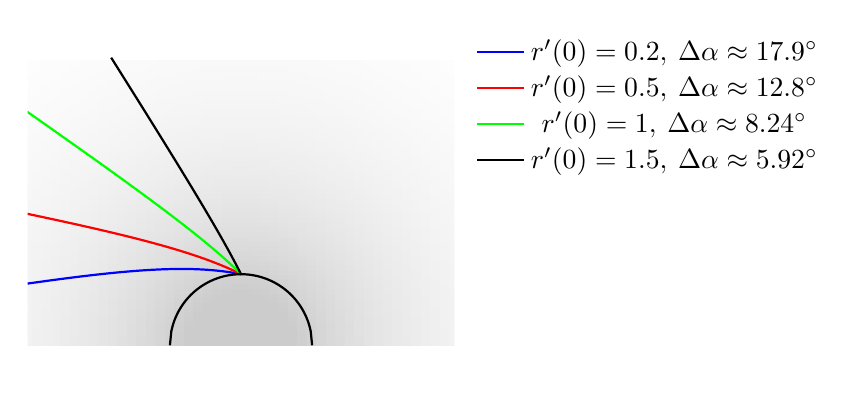
\begin{tikzpicture}
  \begin{axis} [
    axis lines=none, 
    width=7cm, 
    axis equal,
    ticks = none, 
    legend pos = outer north east, 
    legend style={draw=none}, 
    ymin = 0,
    ymax = 4,
    xmin = -3, 
    xmax = 3, 
    zmin = 1,
    zmax = 2,
    %colorbar, 
    colormap={traditionalpm3d}{color=(white) color=(llGray) color=(lGray) color=(lGray)},
    view={0}{90}
  ]  
    \addplot3[surf, domain=-4:4, y domain=0:4, shader=flat, samples=61, forget plot] {1 + 1 * exp(-(sqrt(x^2+y^2)-1)/2)};  
    %f'(0)=0,2
    \addplot [mark = none, thick, color=blue] coordinates {
      (0.00000,1.00000)(-0.01332,1.00264)(-0.02671,1.00523)(-0.04019,1.00778)(-0.05374,1.01028)(-0.09766,1.01802)(-0.14254,1.02531)(-0.18851,1.03217)(-0.23567,1.03858)(-0.28418,1.04453)(-0.33419,1.05001)(-0.38587,1.05501)(-0.43940,1.05950)(-0.49500,1.06345)(-0.55289,1.06684)(-0.61334,1.06963)(-0.67664,1.07177)(-0.74314,1.07321)(-0.81322,1.07389)(-0.88734,1.07372)(-0.96600,1.07263)(-1.04982,1.07052)(-1.13952,1.06724)(-1.23592,1.06265)(-1.34006,1.05657)(-1.45317,1.04879)(-1.57672,1.03902)(-1.71256,1.02692)(-1.86302,1.01211)(-2.03105,0.99406)(-2.22032,0.97204)(-2.43583,0.94521)(-2.68435,0.91244)(-2.97519,0.87217)(-3.32034,0.82190)(-3.73947,0.75864)(-4.26247,0.67763)(-4.66896,0.61339)(-5.15258,0.53572)(-5.74058,0.44042)(-6.47383,0.32098)(-7.07070,0.22331)(-7.78451,0.10590)(-8.65695,-0.03780)(-9.75048,-0.21781)(-10.64136,-0.36457)(-11.70941,-0.54087)(-13.01771,-0.75678)(-14.66075,-1.02765)(-16.00049,-1.24854)(-17.60807,-1.51390)(-19.57873,-1.83911)(-22.05519,-2.24749)(-24.04608,-2.57581)(-26.42972,-2.96917)(-29.34303,-3.44988)(-32.99002,-4.05137)(-34.44359,-4.29116)(-36.03173,-4.55315)(-37.77414,-4.84060)(-39.69468,-5.15743)
    };
    \addlegendentry{$r'(0)=0.2, \: \Delta \alpha \approx 17.9^\circ$};
    
    %f'(0)=0.5
    \addplot [mark = none, thick, color=red] coordinates {
      (0.00000,1.00000)(-0.02287,1.01133)(-0.04628,1.02273)(-0.07026,1.03420)(-0.09484,1.04575)(-0.13129,1.06249)(-0.16915,1.07944)(-0.20856,1.09662)(-0.24964,1.11404)(-0.29253,1.13176)(-0.33741,1.14978)(-0.38445,1.16816)(-0.43386,1.18693)(-0.48586,1.20614)(-0.54073,1.22583)(-0.59876,1.24607)(-0.66027,1.26690)(-0.72567,1.28841)(-0.79538,1.31068)(-0.86993,1.33379)(-0.94992,1.35785)(-1.03605,1.38301)(-1.12913,1.40939)(-1.23016,1.43719)(-1.34033,1.46661)(-1.46106,1.49793)(-1.59408,1.53143)(-1.74156,1.56753)(-1.90621,1.60674)(-2.09152,1.64973)(-2.30177,1.69721)(-2.54287,1.75035)(-2.82274,1.81070)(-3.15233,1.88043)(-3.54591,1.96187)(-4.02657,2.05985)(-4.62950,2.18150)(-5.10124,2.27585)(-5.66443,2.38767)(-6.35138,2.52357)
    };
    \addlegendentry{$r'(0)=0.5, \: \Delta \alpha \approx 12.8^\circ$};
    
    %f'(0) = 1
    \addplot [mark = none, thick, color=green] coordinates {
      (0.00000,1.00000)(-0.02159,1.02144)(-0.04413,1.04355)(-0.06769,1.06635)(-0.09234,1.08990)(-0.11988,1.11587)(-0.14885,1.14283)(-0.17938,1.17085)(-0.21158,1.20002)(-0.24561,1.23044)(-0.28162,1.26222)(-0.31980,1.29548)(-0.36035,1.33036)(-0.40350,1.36702)(-0.44952,1.40562)(-0.49869,1.44638)(-0.55136,1.48951)(-0.60791,1.53528)(-0.66881,1.58400)(-0.73457,1.63602)(-0.80580,1.69175)(-0.88324,1.75168)(-0.96772,1.81638)(-1.06026,1.88654)(-1.16211,1.96301)(-1.27477,2.04682)(-1.40005,2.13916)(-1.54024,2.24163)(-1.69827,2.35624)(-1.87786,2.48554)(-2.08370,2.63268)(-2.32226,2.80216)(-2.60238,3.00014)(-2.93643,3.23523)(-3.34070,3.51823)(-3.84233,3.86838)(-4.48359,4.31531)(-4.95937,4.64639)(-5.52919,5.04235)(-6.22631,5.52657)(-7.10070,6.13397)(-7.94788,6.72246)(-8.99750,7.45079)(-10.34128,8.38345)(-12.12876,9.62479)
    };
    \addlegendentry{$r'(0)=1, \: \Delta \alpha \approx 8.24^\circ$};
       
    %f'(0) = 1.5
    \addplot [mark = none, thick, color=black] coordinates {
      (0.00000,1.00000)(-0.01361,1.02708)(-0.02797,1.05537)(-0.04315,1.08496)(-0.05920,1.11595)(-0.07620,1.14845)(-0.09421,1.18258)(-0.11334,1.21846)(-0.13366,1.25625)(-0.15530,1.29610)(-0.17836,1.33821)(-0.20298,1.38278)(-0.22931,1.43004)(-0.25752,1.48025)(-0.28781,1.53371)(-0.32040,1.59077)(-0.35553,1.65182)(-0.39350,1.71730)(-0.43465,1.78774)(-0.47937,1.86375)(-0.52812,1.94605)(-0.58146,2.03548)(-0.64001,2.13305)(-0.70457,2.23995)(-0.77608,2.35768)(-0.85569,2.48804)(-0.94482,2.63321)(-1.04524,2.79599)(-1.15925,2.97998)(-1.28981,3.18983)(-1.44064,3.43132)(-1.61699,3.71275)(-1.82607,4.04553)
    };        
    \addlegendentry{$r'(0)=1.5, \: \Delta \alpha \approx 5.92^\circ$};
    
    %draw Earth
    \addplot [domain=-1:1, mark=none, black, samples=101, name path=earth, thick] {sqrt(1 - x^2)};
  \end{axis}   
\end{tikzpicture}
\caption{Nummerische L"osung der Exponentiellen Approximation mit $\mu = 1, \: \sigma = 0.5$. 
\label{fig:sphaerisches_modell2}}
\end{figure}

\begin{figure}
\centering
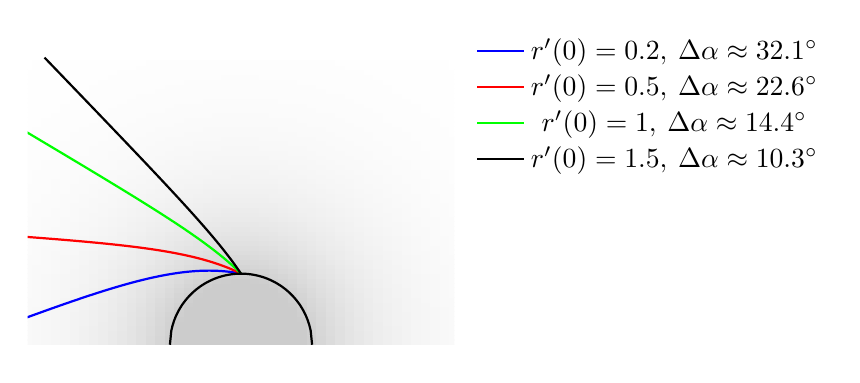
\begin{tikzpicture}
  \begin{axis} [
    axis lines=none, 
    width=7cm, 
    axis equal,
    ticks = none,  
    legend pos = outer north east, 
    legend style={draw=none}, 
    ymin = 0,
    ymax = 4,
    xmin = -3, 
    xmax = 3, 
    zmin = 1,
    zmax = 2,
    %colorbar, 
    colormap={traditionalpm3d}{color=(white) color=(llGray) color=(lGray) color=(lGray) color=(lGray) color=(lGray)},
    view={0}{90}
  ]  
    \addplot3[surf, domain=-4:4, y domain=0:4, shader=flat, samples=61, forget plot] {1 + 1 * exp(-(sqrt(x^2+y^2)-1))};  
    %\addlegendentry{$n(r)$};
    %f'(0)=0,2
    \addplot [mark = none, thick, color=blue] coordinates {
      (0.00000,1.00000)(-0.01801,1.00352)(-0.03615,1.00689)(-0.05442,1.01012)(-0.07284,1.01321)(-0.11443,1.01957)(-0.15680,1.02520)(-0.19999,1.03007)(-0.24407,1.03417)(-0.28911,1.03749)(-0.33517,1.03999)(-0.38232,1.04165)(-0.43065,1.04243)(-0.48026,1.04231)(-0.53123,1.04124)(-0.58369,1.03918)(-0.63774,1.03607)(-0.69354,1.03186)(-0.75122,1.02649)(-0.81095,1.01989)(-0.87293,1.01197)(-0.93737,1.00264)(-1.00451,0.99180)(-1.07463,0.97932)(-1.14805,0.96508)(-1.22513,0.94892)(-1.30629,0.93066)(-1.39204,0.91009)(-1.48295,0.88697)(-1.57972,0.86101)(-1.68316,0.83188)(-1.79427,0.79918)(-1.91426,0.76242)(-2.04464,0.72103)(-2.18719,0.67425)(-2.34428,0.62119)(-2.51893,0.56071)(-2.71505,0.49133)(-2.93756,0.41105)(-3.19352,0.31729)(-3.49277,0.20641)(-3.68095,0.13615)(-3.88930,0.05800)(-4.12164,-0.02945)(-4.38284,-0.12803)
    };
    \addlegendentry{$r'(0) = 0.2, \: \Delta \alpha \approx 32.1^\circ$};
         
    %f'(0)=0.5
    \addplot [mark = none, thick, color=red] coordinates {
      (0.00000,1.00000)(-0.02913,1.01430)(-0.05912,1.02850)(-0.09001,1.04260)(-0.12186,1.05660)(-0.15622,1.07112)(-0.19174,1.08553)(-0.22848,1.09983)(-0.26652,1.11403)(-0.30594,1.12812)(-0.34683,1.14210)(-0.38928,1.15598)(-0.43341,1.16975)(-0.47931,1.18342)(-0.52714,1.19699)(-0.57702,1.21047)(-0.62912,1.22384)(-0.68363,1.23713)(-0.74072,1.25033)(-0.80064,1.26345)(-0.86364,1.27649)(-0.93000,1.28947)(-1.00004,1.30239)(-1.07415,1.31527)(-1.15276,1.32813)(-1.23636,1.34098)(-1.32554,1.35386)(-1.42096,1.36679)(-1.52345,1.37982)(-1.63395,1.39301)(-1.75359,1.40640)(-1.88375,1.42009)(-2.02615,1.43419)(-2.18287,1.44884)(-2.35647,1.46418)(-2.55025,1.48045)(-2.76851,1.49798)(-3.02833,1.51805)(-3.32895,1.54037)(-3.68221,1.56589)(-4.10493,1.59591)
    };
    \addlegendentry{$r'(0) = 0.5, \: \Delta \alpha \approx 22.6^\circ$};
          
    %f'(0) = 1
    \addplot [mark = none, thick, color=green] coordinates {
      (0.00000,1.00000)(-0.02171,1.02148)(-0.04437,1.04344)(-0.06804,1.06590)(-0.09278,1.08889)(-0.11864,1.11245)(-0.14571,1.13661)(-0.17405,1.16141)(-0.20374,1.18689)(-0.23488,1.21311)(-0.26756,1.24010)(-0.30190,1.26793)(-0.33801,1.29666)(-0.37602,1.32636)(-0.41609,1.35711)(-0.45837,1.38900)(-0.50306,1.42213)(-0.55035,1.45662)(-0.60048,1.49258)(-0.65371,1.53016)(-0.71034,1.56953)(-0.77071,1.61088)(-0.83520,1.65443)(-0.90426,1.70043)(-0.97843,1.74919)(-1.05829,1.80105)(-1.14458,1.85642)(-1.23812,1.91579)(-1.33995,1.97976)(-1.45126,2.04905)(-1.57354,2.12449)(-1.70858,2.20718)(-1.85867,2.29845)(-2.02663,2.40001)(-2.21601,2.51391)(-2.43150,2.64296)(-2.67932,2.79091)(-2.96782,2.96277)(-3.30784,3.16476)(-3.71579,3.40682)(-4.21556,3.70328)
    }; 
    \addlegendentry{$r'(0) = 1, \: \Delta \alpha \approx 14.4^\circ$}; 
          
    %f'(0) = 1.5
    \addplot [mark = none, thick, color=black] coordinates {
      (0.00000,1.00000)(-0.01534,1.02283)(-0.03140,1.04634)(-0.04821,1.07057)(-0.06581,1.09556)(-0.08426,1.12135)(-0.10360,1.14799)(-0.12389,1.17554)(-0.14518,1.20404)(-0.16755,1.23357)(-0.19106,1.26418)(-0.21579,1.29596)(-0.24183,1.32898)(-0.26927,1.36333)(-0.29821,1.39912)(-0.32877,1.43646)(-0.36107,1.47546)(-0.39525,1.51627)(-0.43148,1.55905)(-0.46992,1.60396)(-0.51078,1.65121)(-0.55427,1.70102)(-0.60066,1.75363)(-0.65023,1.80935)(-0.70331,1.86851)(-0.76029,1.93149)(-0.82160,1.99875)(-0.88775,2.07080)(-0.95936,2.14828)(-1.03714,2.23191)(-1.12193,2.32256)(-1.21474,2.42128)(-1.31681,2.52937)(-1.42967,2.64838)(-1.55514,2.78022)(-1.69555,2.92731)(-1.85390,3.09277)(-2.03399,3.28060)(-2.24065,3.49573)(-2.48057,3.74517)(-2.76287,4.03847)
    };        
    \addlegendentry{$r'(0) = 1.5, \: \Delta \alpha \approx 10.3^\circ$};
          
    %draw Earth
    \addplot [domain=-1:1, mark=none, black, samples=101, name path=earth, thick] {sqrt(1 - x^2)};
  \end{axis}   
\end{tikzpicture}

\caption{Nummerische L"osung der Exponentiellen Approximation mit $\mu = 1, \: \sigma = 1$. \label{fig:sphaerisches_modell3} }
\end{figure}

\newpage

\subsection{Spezialfall: geschlossener Kreis}
Beim betrachten der Resultate f"allt auf, dass es m"oglicherweise eine Kombination aus Anfangsbedingungen und der Brechzahl das Licht in einem Kreis um den Planeten bricht. 
Um diese Bedingungen zu finden, starten wir mit der Gleichung \ref{eq:sphere_origin}:

$$\Rightarrow n'_r + n - \frac{n r r'' - n r'^2}{r'^2 + r^2} = 0$$

Bei diesem Spezialfall ist $r''(\varphi) = 0$, $r'(\varphi) = 0$. 
Setzen wir nun diese Bedingungen in die Gleichung ein, erhalten wir:

$$n'_r + n = 0 \quad \Rightarrow \quad n'_r(r) = -n(r)$$

Dies ist nun ebenfalls eine Differentialgleichung, welche die L"osung $n(r) = C \cdot e^{-r}$ hat.
Alle diese L"osungen haben die Eigenschaft, dass man bei dieser Verteilung der Brechzahl ein waagerechter Lichtstrahl auf jeder H"ohe in einen geschlossenen Kreis gebrochen wird.
Da diese L"osung die Bedingung $n(r) \geq 1$ jedoch nicht erf"ullt, gibt es keine m"ogliche Verteilung der Brechzahlen, bei der auf jeder H"ohe der waagrechte Lichtstrahl zu einem Kreis gebrochen wird. 
Jedoch ist es m"oglich, dass diese Bedingung auf genau einer H"ohe zutrifft. 
Wir untersuchen wieder die exponentielle Approximation mit:
$$n(r) = 1 + \mu \cdot e^{-\sigma (r-r_0)} \qquad n'(r) = -\mu \sigma \cdot e^{-\sigma (r-r_0)}$$

Wir setzen diese Funktionen nun in die obrige Bedingung ein und erhalten:

$$\mu \sigma \cdot e^{-\sigma (r-r_0)} = 1 + \mu \cdot e^{-\sigma (r-r_0)} \quad \Rightarrow \quad \mu \cdot e^{-\sigma (r-r_0)} \cdot (\sigma - 1) = 1$$

$$\mu = \frac{e^{\sigma (r-r_0)}}{\sigma - 1}$$

Wenn wir $r = r_0$ und $\sigma = 2$ festhalten, ergibt sich $\mu = 1$. 
Auch die Simulation best"atigt, dass in diesem Fall das Licht in einem Kreis gebrochen wird.
In der Simulation wurde auch ein leicht verf"alschter Lichtstrahl dargestellt, mit 0.01 Abweichung. 
Da es in der Luft immer viele Unregelm"assigkeiten des Druckes, der Temperatur und der Luftfeuchtigkeit gibt, soll dieser Lichtstrahl zeigen, wie sich ein solcher Fehler auf den Verlauf auswirkt.

Wie man erkennen kann ist dieser Lichtstrahl bis $90^\circ$ nicht vom anderen zu unterscheiden.
Bei der Simulation ist jedoch der Radius mit $r_0=1$ sehr klein gewählt worden. 
Wenn der Radius gr"osser gemacht wird ($r_0 = 100$), so  verl"asst der Lichtstrahl viel fr"uher den pfad (Abbildung \ref{fig:sphere_special2}). 

Jedoch ist eine solch extreme Athmosph"are nicht realistisch. 
Bei $r = r_0$ betr"agt die Brechzahl $n(r_0) = 1 + \mu = 2$. 
Diese Brechzahl ist nicht realistisch. 
Es braucht also ein anderes Modell, mit dem man diesen Effekt erzeugen kann.

Die Brechzahl der Luft ist nicht nur vom Druck abh"angig, sondern auch von der Luftfeuchtigkeit. 
dazu wird folgende quadratische Approximation verwendet:

$$n(r) = \left\{ \begin{array}{ll} 1 + \mu \cdot (r_0 - r)^2 & \text{wenn } r < r_0 \\ 1 & \text{sonst} \end{array} \right. \quad n'_r(r) = \left\{ \begin{array}{ll} 2\mu \cdot (r - r_0) & \text{wenn } r < r_0 \\ 0 & \text{sonst} \end{array} \right.$$

Nun l"osen wir die obere Bedingung $-n'_r = n $, wenn $r < r_0$:

$$2\mu \cdot (r_0 - r) = 1 + \mu(r_0 - r)^2$$

Wenn wir nun f"ur $(r_0 - r) = 1$ einsetzen, erhalten wir $\mu = 1$. 
Bei der Simulation mit diesen Bedingungen ist ersichtlich, dass in einen Kreis gebrochen wird (Abbildung \ref{fig:sphere_special3}). 
Wenn aber wie erneut der Fehler Simuliert wird, ist die Abweichung viel kleiner als bei der exponentiellen Approximation. 
Nun erh"ohen wir ebenfalls den Radius $r_0$ und wiederholen die Simulation. 
Bei $r_0 = 1000$ ist der Lichtstrahl immer noch f"ur lange Zeit auf dem idealen Kreis (Abbildung \ref{fig:sphere_special4}). 
Bei dieser Approximation ist es also möglich, dass sich ein Lichtstrahl f"ur kurze Zeit in einen Kreisbogen bricht, auch bei gr"osserem $r_0$.

\begin{figure}
  \centering
  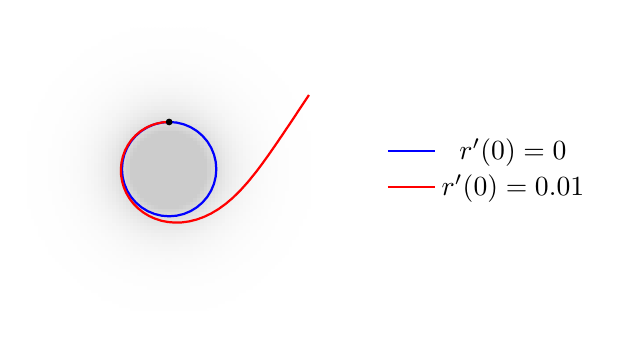
\begin{tikzpicture}
        \begin{axis} [
          axis lines=none, 
          width=6cm, 
          axis equal,
          ticks = none,  
          legend style={at={(1.1,0.5)}, anchor=west, draw=none}, 
          ymin = -3,
          ymax = 3,
          xmin = -3, 
          xmax = 3, 
          zmin = 1,
          zmax = 2,
          %colorbar, 
          colormap={traditionalpm3d}{color=(white) color=(lGray) color=(lGray) color=(lGray) color=(lGray) color=(lGray)},
          view={0}{90}
        ]  
          \addplot3[surf, domain=-3:3, y domain=-3:3, shader=flat, samples=81, forget plot] {1 + 1 * exp(-(2*sqrt(x^2+y^2)-1))};  
          %\addlegendentry{$n(r)$};
          %f'(0)=0
          \addplot [mark = none, thick, color=blue] coordinates {
            (0.00000,1.00000)(-0.15643,0.98769)(-0.30902,0.95106)(-0.45399,0.89101)(-0.58779,0.80902)(-0.70711,0.70711)(-0.80902,0.58779)(-0.89101,0.45399)(-0.95106,0.30902)(-0.98769,0.15643)(-1.00000,0.00000)(-0.98769,-0.15643)(-0.95106,-0.30902)(-0.89101,-0.45399)(-0.80902,-0.58779)(-0.70711,-0.70711)(-0.58779,-0.80902)(-0.45399,-0.89101)(-0.30902,-0.95106)(-0.15643,-0.98769)(-0.00000,-1.00000)(0.15643,-0.98769)(0.30902,-0.95106)(0.45399,-0.89101)(0.58779,-0.80902)(0.70711,-0.70711)(0.80902,-0.58779)(0.89101,-0.45399)(0.95106,-0.30902)(0.98769,-0.15643)(1.00000,-0.00000)(0.98769,0.15643)(0.95106,0.30902)(0.89101,0.45399)(0.80902,0.58779)(0.70711,0.70711)(0.58779,0.80902)(0.45399,0.89101)(0.30902,0.95106)(0.15643,0.98769)(0.00000,1.00000)
          };
          \addlegendentry{$r'(0) = 0$};
          
          %f'(0)=0.01
          \addplot [mark = none, thick, color=red] coordinates {
            (0.00000,1.00000)(-0.12980,0.99286)(-0.25776,0.96893)(-0.38171,0.92862)(-0.49959,0.87255)(-0.60942,0.80165)(-0.70937,0.71707)(-0.79777,0.62017)(-0.87315,0.51253)(-0.93426,0.39588)(-0.98008,0.27209)(-1.00983,0.14313)(-1.02298,0.01104)(-1.01929,-0.12208)(-0.99875,-0.25418)(-0.96162,-0.38319)(-0.90837,-0.50715)(-0.83973,-0.62418)(-0.75662,-0.73250)(-0.66013,-0.83051)(-0.55152,-0.91676)(-0.43215,-0.98999)(-0.30348,-1.04909)(-0.16700,-1.09320)(-0.02422,-1.12159)(0.12339,-1.13373)(0.27444,-1.12923)(0.42765,-1.10781)(0.58193,-1.06927)(0.73643,-1.01342)(0.89054,-0.93996)(1.04407,-0.84843)(1.19734,-0.73804)(1.35138,-0.60737)(1.50773,-0.45385)(1.66973,-0.27355)(1.84298,-0.05971)(1.96559,0.10267)(2.09982,0.28898)(2.25133,0.50660)(2.42853,0.76699)(2.53821,0.93037)(2.66132,1.11504)(2.80161,1.32643)(2.96417,1.57197)
          };
          \addlegendentry{$r'(0) = 0.01$};

          \draw [fill=black] (axis cs:0,1) circle (1pt);           
          
          \end{axis}   
      \end{tikzpicture}  
  \caption{Nummersiche L"osung der exponentiellen Approximation mit $r(0) = r_0 = 1$, $r'(0) = 0$, $\sigma = 2$, $\mu = 1$. \label{fig:sphere_special1}}

\end{figure}

\begin{figure}
  \centering
  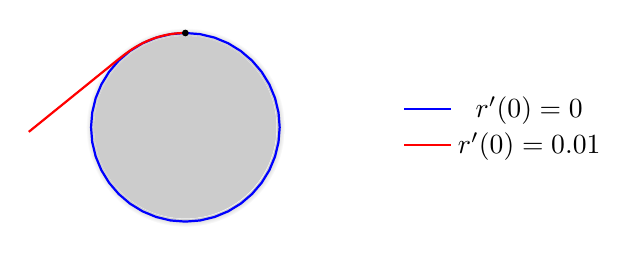
\begin{tikzpicture}
        \begin{axis} [
          axis lines=none, 
          width=6cm, 
          axis equal,
          ticks = none,  
          legend style={at={(1.1,0.5)}, anchor=west, draw=none}, 
          ymin = -150,
          ymax = 150,
          xmin = -150, 
          xmax = 150, 
          zmin = 1,
          zmax = 2,
          %colorbar, 
          colormap={traditionalpm3d}{color=(white) color=(lGray) color=(lGray) color=(lGray) color=(lGray) color=(lGray)},
          view={0}{90}
        ]  
          %\addplot3[surf, domain=-150:-70, y domain=-150:150, shader=flat, samples=81, forget plot] {1 + 1 * exp(-2*(sqrt(x^2+y^2)-100))};  
          \draw [draw=none, fill=lGray] (axis cs:0,0) circle (33pt);  
          \shade[even odd rule,ring shading={from lGray at 33pt to white at 36pt}]
  (axis cs:0,0) circle (33pt) circle (36pt);
          %\addlegendentry{$n(r)$};
          %f'(0)=0
          \addplot [mark = none, thick, color=blue] coordinates {
            (0.00000,100.00000)(-15.64345,98.76883)(-30.90170,95.10565)(-45.39905,89.10065)(-58.77853,80.90170)(-70.71068,70.71068)(-80.90170,58.77853)(-89.10065,45.39905)(-95.10565,30.90170)(-98.76883,15.64345)(-100.00000,0.00000)(-98.76883,-15.64345)(-95.10565,-30.90170)(-89.10065,-45.39905)(-80.90170,-58.77853)(-70.71068,-70.71068)(-58.77853,-80.90170)(-45.39905,-89.10065)(-30.90170,-95.10565)(-15.64345,-98.76883)(-0.00000,-100.00000)(15.64345,-98.76883)(30.90170,-95.10565)(45.39905,-89.10065)(58.77853,-80.90170)(70.71068,-70.71068)(80.90170,-58.77853)(89.10065,-45.39905)(95.10565,-30.90170)(98.76883,-15.64345)(100.00000,-0.00000)(98.76883,15.64345)(95.10565,30.90170)(89.10065,45.39905)(80.90170,58.77853)(70.71068,70.71068)(58.77853,80.90170)(45.39905,89.10065)(30.90170,95.10565)(15.64345,98.76883)(0.00000,100.00000)
          };
          \addlegendentry{$r'(0) = 0$};
          
          %f'(0)=0.01
          \addplot [mark = none, thick, color=red] coordinates {
            (0.00000,100.00000)(-2.75512,99.96232)(-5.50816,99.84877)(-8.25704,99.65945)(-10.99968,99.39454)(-13.73400,99.05427)(-16.45795,98.63893)(-19.16948,98.14889)(-21.86655,97.58457)(-24.83804,96.87257)(-27.78659,96.07065)(-30.70957,95.17975)(-33.60441,94.20094)(-36.40398,93.16060)(-39.17210,92.03878)(-41.90675,90.83701)(-44.60607,89.55703)(-47.22896,88.22171)(-49.81483,86.81471)(-52.36296,85.33870)(-54.87321,83.79685)(-57.31713,82.21217)(-59.72629,80.57104)(-62.10361,78.87857)(-64.45352,77.14051)(-66.70407,75.42338)(-68.94185,73.67578)(-71.17485,71.90315)(-73.41120,70.10955)(-76.13995,67.90859)(-78.89590,65.67960)(-81.68846,63.41934)(-84.52594,61.12262)(-87.92412,58.37178)(-91.40873,55.55090)(-94.99475,52.64789)(-98.69878,49.64942)(-102.53924,46.54059)(-106.53665,43.30458)(-110.71453,39.92239)(-115.09991,36.37236)(-119.72392,32.62940)(-124.62209,28.66415)(-129.83697,24.44237)(-135.41925,19.92349)(-142.02863,14.57418)(-149.24574,8.73133)(-157.19207,2.29774)(-166.02222,-4.84984)
          };
          \addlegendentry{$r'(0) = 0.01$};

          \draw [fill=black] (axis cs:0,100) circle (1pt);         
          
          \end{axis}   
      \end{tikzpicture}
  \caption{Nummerische L"osung der exponentielle Approximation mit $r(0) = r_0 = 100$, $\sigma = 2$, $\mu = 1$. \label{fig:sphere_special2}} 
  
\end{figure}

\begin{figure}
  \centering
  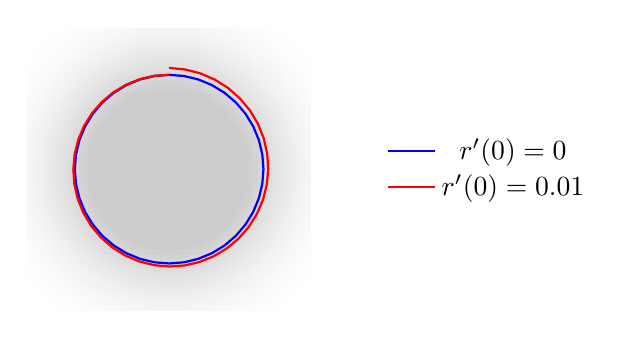
\begin{tikzpicture}
    \begin{axis} [
          axis lines=none, 
          width=6cm, 
          axis equal,
          ticks = none,  
          legend style={at={(1.1,0.5)}, anchor=west, draw=none}, 
          ymin = -1.5,
          ymax = 1.5,
          xmin = -1.5, 
          xmax = 1.5, 
          zmin = 1,
          zmax = 2,
          %colorbar, 
          colormap={traditionalpm3d}{color=(white) color=(lGray) color=(lGray) color=(lGray)},
          view={0}{90}
        ]  
          \addplot3[surf, domain=-1.5:1.5, y domain=-1.5:1.5, shader=flat, samples=61, forget plot] {1 + (2-sqrt(x^2+y^2))^2};  
          %\draw [draw=none, fill=lGray] (axis cs:0,0) circle (33pt);  
          %\shade[even odd rule,ring shading={from lGray at 33pt to white at 36pt}]
            %(axis cs:0,0) circle (33pt) circle (36pt);
          %\addlegendentry{$n(r)$};
          %f'(0)=0
          \addplot [mark = none, thick, color=blue] coordinates {
            (0.00000,1.00000)(-0.15643,0.98769)(-0.30902,0.95106)(-0.45399,0.89101)(-0.58779,0.80902)(-0.70711,0.70711)(-0.80902,0.58779)(-0.89101,0.45399)(-0.95106,0.30902)(-0.98769,0.15643)(-1.00000,0.00000)(-0.98769,-0.15643)(-0.95106,-0.30902)(-0.89101,-0.45399)(-0.80902,-0.58779)(-0.70711,-0.70711)(-0.58779,-0.80902)(-0.45399,-0.89101)(-0.30902,-0.95106)(-0.15643,-0.98769)(-0.00000,-1.00000)(0.15643,-0.98769)(0.30902,-0.95106)(0.45399,-0.89101)(0.58779,-0.80902)(0.70711,-0.70711)(0.80902,-0.58779)(0.89101,-0.45399)(0.95106,-0.30902)(0.98769,-0.15643)(1.00000,-0.00000)(0.98769,0.15643)(0.95106,0.30902)(0.89101,0.45399)(0.80902,0.58779)(0.70711,0.70711)(0.58779,0.80902)(0.45399,0.89101)(0.30902,0.95106)(0.15643,0.98769)(0.00000,1.00000)
          };
          \addlegendentry{$r'(0) = 0$};
          
          %f'(0)=0.01
          \addplot [mark = none, thick, color=red] coordinates {
            (0.00000,1.00000)(-0.15668,0.98924)(-0.30999,0.95405)(-0.45614,0.89522)(-0.59149,0.81412)(-0.71268,0.71268)(-0.81668,0.59335)(-0.90086,0.45901)(-0.96309,0.31293)(-1.00177,0.15866)(-1.01586,0.00000)(-1.00494,-0.15917)(-0.96921,-0.31491)(-0.90946,-0.46339)(-0.82709,-0.60091)(-0.72406,-0.72406)(-0.60285,-0.82975)(-0.46638,-0.91532)(-0.31797,-0.97860)(-0.16123,-1.01796)(-0.00000,-1.03235)(0.16176,-1.02134)(0.32008,-0.98511)(0.47105,-0.92448)(0.61091,-0.84085)(0.73620,-0.73620)(0.84379,-0.61305)(0.93096,-0.47435)(0.99549,-0.32346)(1.03573,-0.16404)(1.05060,-0.00000)(1.03964,0.16466)(1.00301,0.32590)(0.94154,0.47974)(0.85662,0.62237)(0.75026,0.75026)(0.62497,0.86020)(0.48376,0.94942)(0.33001,1.01566)(0.16744,1.05719)(0.00000,1.07288)
          };
          \addlegendentry{$r'(0) = 0.01$};
          \draw [fill=black] (axis cs:0,100) circle (1pt);         
          
          \end{axis}   
      \end{tikzpicture}
  \caption{Nummerische L"osung der quadratischen Approximation mit $r(0) = r_0 = 1$, $mu = 1$. \label{fig:sphere_special3} }
  
\end{figure}

\begin{figure}
  \centering
  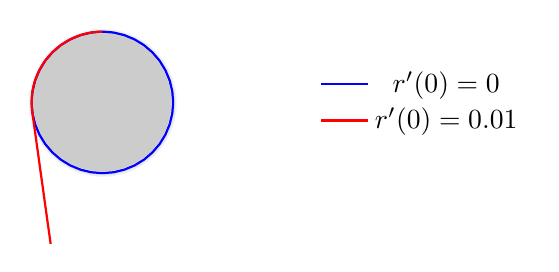
\begin{tikzpicture}
        \begin{axis} [
          axis lines=none, 
          width=6cm, 
          axis equal,
          ticks = none,  
          legend style={at={(1.1,0.5)}, anchor=west, draw=none}, 
          ymin = -2000,
          ymax = 2000,
          xmin = -2000, 
          xmax = 2000, 
          zmin = 1,
          zmax = 2,
          %colorbar, 
          colormap={traditionalpm3d}{color=(white) color=(lGray) color=(lGray) color=(lGray)},
          view={0}{90}
        ]  
          %\addplot3[surf, domain=-1.5:1.5, y domain=-1.5:1.5, shader=flat, samples=61, forget plot] {1 + (2-sqrt(x^2+y^2))^2};  
          \draw [draw=none, fill=lGray] (axis cs:0,0) circle (25pt);  
          \shade[even odd rule,ring shading={from lGray at 25pt to white at 27pt}]
            (axis cs:0,0) circle (25pt) circle (27pt);
          %\addlegendentry{$n(r)$};
          %f'(0)=0
          \addplot [mark = none, thick, color=blue] coordinates {
            (   0,1000)(-156, 988)(-309, 951)(-454, 891)(-588, 809)(-707, 707)(-809, 588)(-891, 454)(-951, 309)(-988, 156)(-1000,   0)(-988,-156)(-951,-309)(-891,-454)(-809,-588)(-707,-707)(-588,-809)(-454,-891)(-309,-951)(-156,-988)(  -0,-1000)( 156,-988)( 309,-951)( 454,-891)( 588,-809)( 707,-707)( 809,-588)( 891,-454)( 951,-309)( 988,-156)(1000,  -0)( 988, 156)( 951, 309)( 891, 454)( 809, 588)( 707, 707)( 588, 809)( 454, 891)( 309, 951)( 156, 988)(   0,1000)
          };
          \addlegendentry{$r'(0) = 0$};
          
          %f'(0)=0.01
          \addplot [mark = none, thick, color=red] coordinates {
            (   0,1000)( -70, 998)(-140, 990)(-208, 978)(-276, 961)(-343, 939)(-408, 913)(-471, 882)(-531, 847)(-589, 808)(-644, 765)(-696, 718)(-745, 667)(-790, 614)(-831, 557)(-867, 498)(-900, 436)(-922, 387)(-942, 336)(-959, 285)(-973, 233)(-980, 198)(-987, 163)(-992, 128)(-996,  93)(-998,  68)(-999,  44)(-1000,  19)(-1000,  -6)(-1000, -23)(-999, -39)(-999, -55)(-998, -72)(-997, -83)(-996, -95)(-995,-106)(-994,-117)(-993,-124)(-992,-130)(-991,-136)(-990,-143)(-990,-145)(-990,-148)(-989,-150)(-989,-153)(-989,-155)(-988,-158)(-988,-160)(-988,-163)(-987,-165)(-987,-168)(-987,-170)(-986,-173)(-984,-186)(-983,-199)(-981,-212)(-979,-225)(-970,-290)(-961,-356)(-951,-425)(-941,-496)(-930,-577)(-918,-662)(-905,-755)(-891,-856)(-876,-967)(-858,-1093)(-838,-1236)(-815,-1404)(-797,-1532)(-777,-1677)(-753,-1845)(-726,-2042)
          };
          \addlegendentry{$r'(0) = 0.01$};
          %\draw [fill=black] (axis cs:0,100) circle (1pt);         
          
          \end{axis}   
      \end{tikzpicture}
  \caption{Nummerische L"osung der quadratischen Approximation mit $r(0) = r_0 = 1000$,  $\mu = 1$. \label{fig:sphere_special4} } 
\end{figure}

TODO: Diskusion dieser Resultate / L"osungen

\section{Modellierung der Athmosph"are der Erde}

In den oben hergeleiteten Gleichungen kommt immer die Brechzahl vor. 
Bei bisherigen Simulationen sind wir von einer (willk"urlichen) Funktion ausgegangen, ohne uns dabei auf die Physik zu st"utzen. 
Nun wollen wir ein m"oglichst realistisches, aber dennoch einfaches Modell f"ur die Atmosph"are der Erde finden.

Die Brechzahl der Luft h"angt von volgenden Faktoren ab:
\begin{itemize}
  \item Wellenl"ange des Lichts: In unserem Modell gehen wir von einer konstanten Wellenl"ange aus. Dieser Effekt wird nicht ber"ucksichtigt.
  \item Wasserfeuchtigkeit: Wasserdampf Anteil in der Luft beeinflusst die Brechzahl relativ stark. Jedoch variiert diese sehr stark mit dem Wetter. Deshalb wird dieser Einfluss vernachl"assigt. 
  \item Luftdruck: Der Luftdruck l"asst sich approximativ relativ gut modellieren. Aus der Physik ist bekannt, dass der Druck bei Gasen mit der H"ohe exponentiell abnimmt. 
  \item Temperatur: Wie in Abbildung \ref{fig:athmosphere_profile} erkennbar ist, ver"andert sich die Temperatur in abh"angigkeit der H"ohe sehr stark. Es ist jedoch sehr schwer, diesen Verlauf zu modellieren. Deshalb wird die Temperatur (vorerst) im Modell vernachl"assigt.
\end{itemize}

\begin{figure}
  \centering
  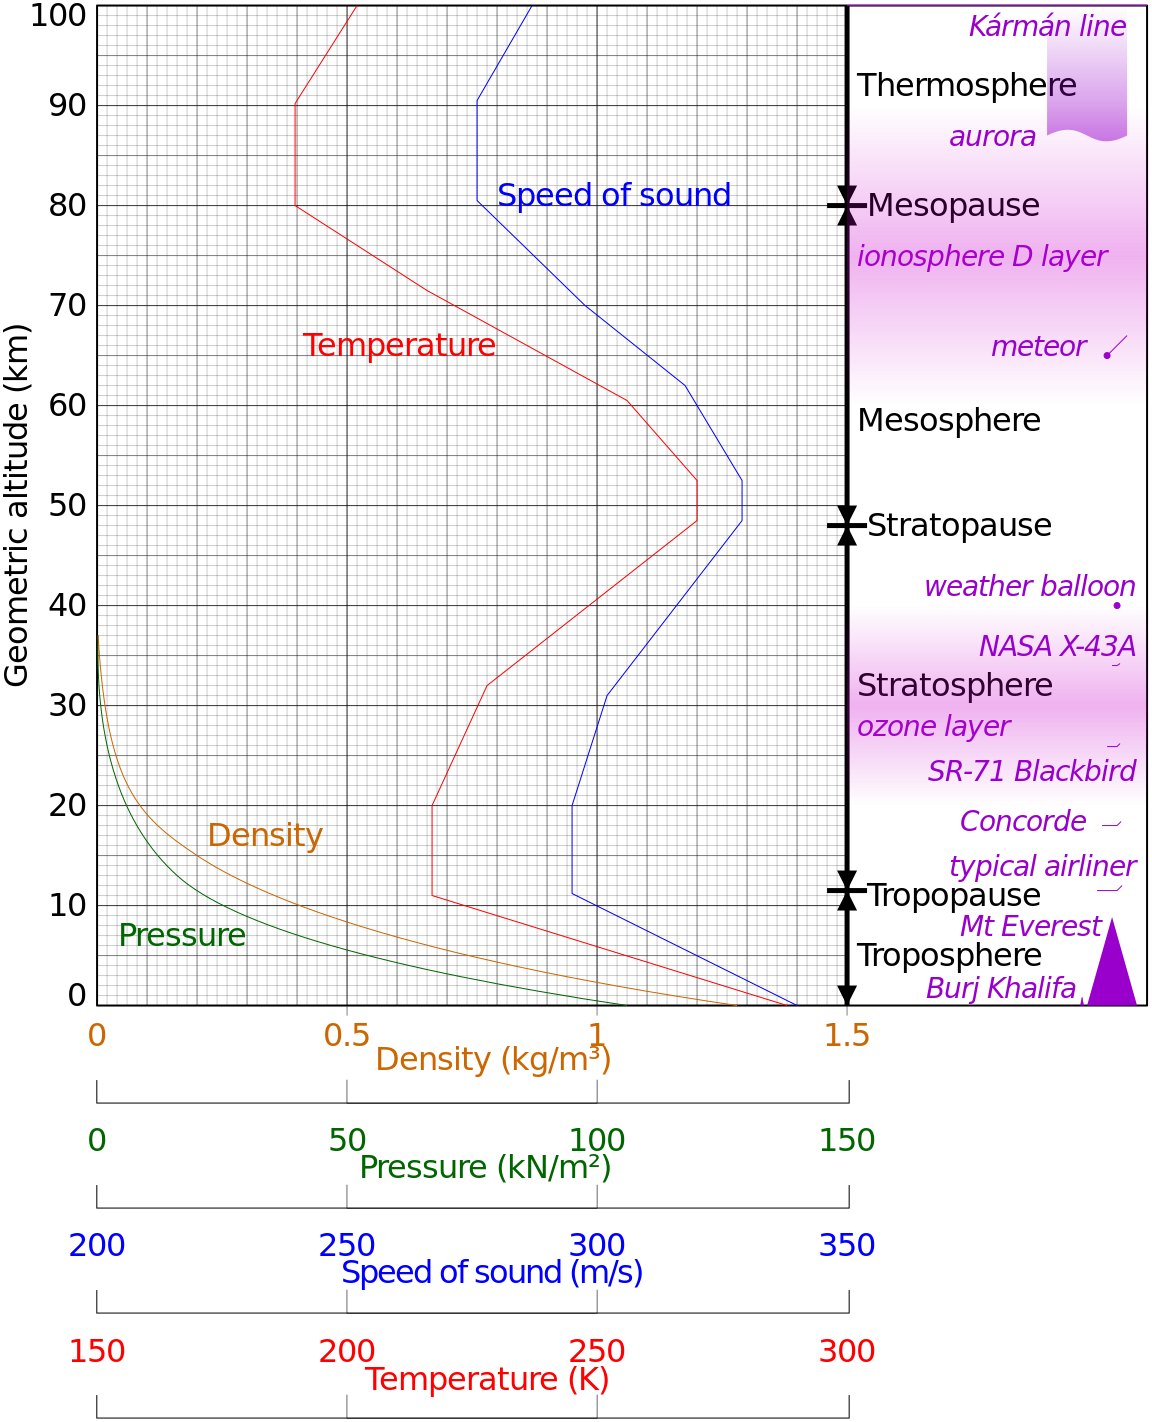
\includegraphics[scale=0.24]{licht/images/athmosphereProfile.png}
  
  \caption{Druck, Dichte, Temperatur und Schallgeschwindigkeit in Abh"angigkeit der H"ohe. \label{fig:athmosphere_profile}}
  %QUELLE: https://en.wikipedia.org/wiki/Atmospheric_temperature
\end{figure}

Dank diesen Vereinfachungen l"asst sich die Brechzahl in Abh"angigkeit folgendermassen beschreiben:

$$n(r) = 1 + \mu \cdot e^{-\sigma (r - r_0)}$$

Der Parameter $r_0$ steht für den Radius der Erdoberfl"ache. 
Bei $r = r_0$ ergibt sich $n(r_0) = n_0 = 1 + \mu$. 
$\sigma$ gibt an, wie schnell die Brechzahl zum tiefsten Wert $n = 1$ geht. 


%Quelle: https://en.wikipedia.org/wiki/List_of_refractive_indices  %Brechzahl
%Quelle: https://en.wikipedia.org/wiki/Earth  % Erdradius


Durch Messungen ist der mittlere Erdradius $r_0 = 6.371 * 10^6$. 
Die Brechzahl auf dieser H"ohe betr"agt: $n_0 = 1.000293$.
Dementsprechend beträgt $\mu = 2.93 * 10^{-3}$. 
Um $\sigma$ abzusch"atzen, wird in der Abbildung \ref{fig:athmosphere_profile} Funktion der Dichte untersucht. 
Die H"ohe bei 36.8\% der Maximaldichte (Dichte auf Meeresh"ohe) entspricht $\sigma$. 
Somit wird $\sigma \approx 9 * 10^3$.

Mit diesen Parametern l"asst sich die erneut die L"osung zum Sph"arischen Modell nummerisch Berechnen. 
Aufgrund der Parameter erwarten wir eine sehr schwache Kr"ummung. 
Dies kann man auch an der Abbildung \ref{fig:sphere_real} erkennen. 
Die Vergleichsgr"osse $\Delta \alpha$, welche aus der Simulation resultiert, zeigt erneut, dass der Lichtstrahl st"arker gebrochen wird, wenn er horizontal eintrifft. 

\begin{figure}
  \centering
  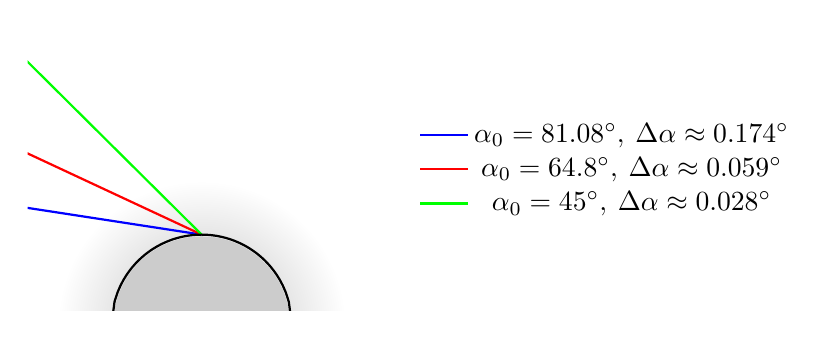
\begin{tikzpicture}
    \begin{axis} [
          axis lines=none, 
          width=6cm, 
          axis equal,
          ticks = none,  
          legend style={at={(1.1,0.5)}, anchor=west, draw=none}, 
          ymin = 1,
          ymax = 21,
          xmin = -10, 
          xmax = 10, 
          %colorbar, 
          colormap={traditionalpm3d}{color=(white) color=(lGray) color=(lGray) color=(lGray)},
          view={0}{90}
        ]  
          %\addplot3[surf, domain=-10000:10000, y domain=0:10000, shader=flat, samples=61, forget plot] {1 + 0.000293*exp()};  
          \draw [draw=none, fill=lGray] (axis cs:0,0) circle (32pt);  
          \shade[even odd rule,ring shading={from llGray at 32pt to white at 52pt}]
            (axis cs:0,0) circle (32pt) circle (52pt);
          %\addlegendentry{$n(r)$};
          %a0 = 8.9
          \addplot [mark = none, thick, color=blue] coordinates {
            (0.0000,6.3710)(-0.0854,6.3842)(-0.1711,6.3974)(-0.2573,6.4106)(-0.3440,6.4240)(-0.4513,6.4405)(-0.5595,6.4571)(-0.6685,6.4738)(-0.7785,6.4907)(-0.9645,6.5193)(-1.1536,6.5484)(-1.3463,6.5780)(-1.5429,6.6082)(-1.7439,6.6391)(-1.9498,6.6707)(-2.1611,6.7032)(-2.3782,6.7365)(-2.6019,6.7709)(-2.8327,6.8064)(-3.0713,6.8430)(-3.3186,6.8810)(-3.5754,6.9205)(-3.8428,6.9616)(-4.1217,7.0044)(-4.4134,7.0493)(-4.7193,7.0963)(-5.0409,7.1457)(-5.3801,7.1978)(-5.7388,7.2529)(-6.1193,7.3114)(-6.5245,7.3736)(-6.9573,7.4401)(-7.4215,7.5115)(-7.9214,7.5883)(-8.4622,7.6714)(-9.0499,7.7617)(-9.6920,7.8603)(-10.3975,7.9688)(-11.1776,8.0886)(-12.0459,8.2220)(-13.0203,8.3718)(-14.0236,8.5260)(-15.1558,8.6999)(-16.4456,8.8981)(-17.9312,9.1264)
          };
          \addlegendentry{$\alpha_0 = 81.08^\circ, \: \Delta \alpha \approx 0.174^\circ$};
          
          %a0 = 1
          \addplot [mark = none, thick, color=red] coordinates {
            (0.0000,6.3710)(-0.1286,6.4312)(-0.2598,6.4922)(-0.3938,6.5548)(-0.5306,6.6187)(-0.6706,6.6841)(-0.8140,6.7510)(-0.9610,6.8196)(-1.1119,6.8900)(-1.2669,6.9623)(-1.4264,7.0367)(-1.5907,7.1134)(-1.7601,7.1924)(-1.9351,7.2741)(-2.1160,7.3585)(-2.3033,7.4459)(-2.4975,7.5365)(-2.6992,7.6307)(-2.9091,7.7286)(-3.1276,7.8306)(-3.3557,7.9370)(-3.5941,8.0482)(-3.8438,8.1648)(-4.1058,8.2870)(-4.3812,8.4155)(-4.6714,8.5509)(-4.9778,8.6939)(-5.3021,8.8452)(-5.6462,9.0058)(-6.0122,9.1766)(-6.4027,9.3588)(-6.8205,9.5538)(-7.2690,9.7631)(-7.7521,9.9885)(-8.2744,10.2322)(-8.8413,10.4967)(-9.4593,10.7851)(-10.1362,11.1010)(-10.8815,11.4488)(-11.7068,11.8339)(-12.6265,12.2630)
          };
          \addlegendentry{$\alpha_0 = 64.8^\circ, \: \Delta \alpha \approx 0.059^\circ$};
          
          %a0 = 1
          \addplot [mark = none, thick, color=green] coordinates {
            (0.0000,6.3710)(-0.1251,6.4954)(-0.2552,6.6245)(-0.3908,6.7592)(-0.5323,6.9000)(-0.6804,7.0470)(-0.8354,7.2010)(-0.9982,7.3626)(-1.1693,7.5326)(-1.3496,7.7117)(-1.5400,7.9008)(-1.7415,8.1009)(-1.9553,8.3133)(-2.1827,8.5392)(-2.4252,8.7801)(-2.6847,9.0378)(-2.9631,9.3143)(-3.2629,9.6121)(-3.5868,9.9338)(-3.9381,10.2827)(-4.3208,10.6629)(-4.7397,11.0790)(-5.2004,11.5365)(-5.7099,12.0426)(-6.2770,12.6058)(-6.9124,13.2371)(-7.6297,13.9495)(-8.4465,14.7607)(-9.3862,15.6941)(-10.4798,16.7807)(-11.7675,18.0594)(-13.3093,19.5904)(-15.1917,21.4606)(-16.8948,23.1527)(-18.9317,25.1753)(-21.4179,27.6443)(-24.5257,30.7319)(-27.1015,33.2910)(-30.1918,36.3598)(-33.9782,40.1202)(-38.7332,44.8440)(-42.6155,48.7007)(-47.2755,53.3287)(-52.9886,59.0030)(-60.1683,66.1352)(-66.0243,71.9524)(-73.0544,78.9346)(-81.6748,87.4967)(-92.5103,98.2602)(-101.2007,106.8927)(-111.6034,117.2249)(-124.3122,129.8480)(-140.2120,145.6417)(-146.2182,151.6076)(-152.7488,158.0944)(-159.8760,165.1737)(-167.6860,172.9313)
          };
          \addlegendentry{$\alpha_0 = 45^\circ, \: \Delta \alpha \approx 0.028^\circ$};
          
      \addplot [thick, mark=none, domain=-6.371:6.371, samples=61, forget plot] { sqrt((6.371)^2-x^2)};      
     
    \end{axis}   
  \end{tikzpicture}
  \caption{Nummerische L"osung des realistischen Modells. \label{fig:sphere_real} } 
\end{figure}
